
\section{Funktionen}\label{Funktionen}
\subsection{Grundfunktionen}
\begin{itemize}
\item Daten von externen API's abfragen
\item Daten von externen API's anzeigen (Widgets)
\item Einstellungen über ein Web Frontend vornhemen
\item Schnittstelle für andere Erweiterungen (externe Clients)
\item ...und natürlich auch die Grundfunktion spiegeln nicht vergessen
\end{itemize}

%
%\begin{itemize}
%\item Google Kalender
%\item Todoist
%\item BVG
%\item Wetter
%\end{itemize}
\subsection{Extras}
\begin{itemize}
\item Face Recognition
\item Voice Control
\item Bewegungssensor
\item Motion Control
\end{itemize}

\subsection{Face Recognition}
Ein SmartMirror mit einem einzigen Ansichts Fenster und auch nur einem Kalendar wäre nicht das optimalste in jedem Haushalt, denn jedes Familienmitglied oder jeder Mitbewohner hat seine eigenen Termine und Kalendareinträge. Eine mögliche Lösung wäre das jeder seinen eigenen SmartMirror besitzt, es wäre jedoch nicht effizienteste und effektivste Lösung. Daher wäre die beste Lösung die "Face-Recognition". Dieser hat die Funktionalität, mithilfe von Machine Learning sich das Gesicht zu merken und es auch wiederzuerkennen. Es könnte dadurch für jede Person im Haushalt ein Profil angelegt werden, und alles was an Modulen und Einstellungen getätigt wird innerhalb dieses Profiles zuspeichern. Je nachdem wer dann vor dem Spiegel steht, dessen Profil, die jeweiligen Module werden, geladen und im Spiegel dargestellt, als Beispiel der Kalendar der jeweiligen Person. 
 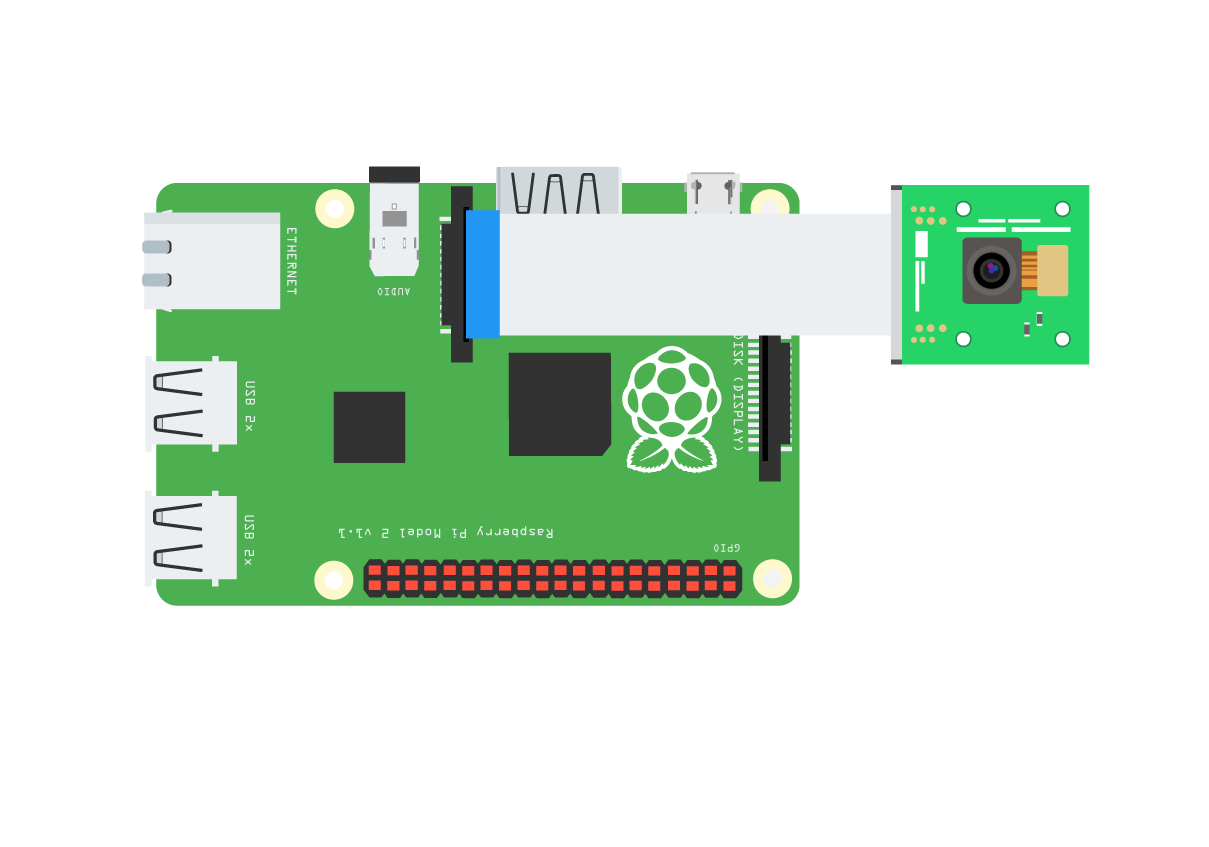
\includegraphics[width=100]{pictures/raspberry-pi-camera-2.png}
 \caption{Raspberry-pi Kamera}

\subsection{Voice Control}
Was gebe es noch cooleres als ein Voice Control System im Spiegel? Während man am Haare fönen ist oder der Bart mal wieder rasiert werden muss und nebenbei Aufgaben, wie Kalendar Einträge & Todo-Aufgaben hinzufügen zu lassen oder auch die Abfahrten der lokalen Öffentlichen Verkehrsmittel, wie Bus und Bahn,  abfragen kann, sowie jegliche Staumeldungen auf der Autobahn, mit nur einem Satz erledigt werden können. Als Hardware wird lediglich ein Mikrof und ein Latusprecher benötigt.

\subsection{Bewgungssensor}
Um unseren SmartMirror möglichst effizient zu gestalten wäre die Verwendung eines Bewegungssensor sehr angebracht. Es sollte so funktionieren, dass sobald jemand vor dem Spiegel steht, der Spiegel aus dem Stand-By Modus zum Aktiven Modus wechselt. Somit wäre der Spiegel nicht die ganze Zeit über an und würde den Stromverbrauch deutlich senken. Der wäre an Bodenplatte des Spiegels zu befestigen. 
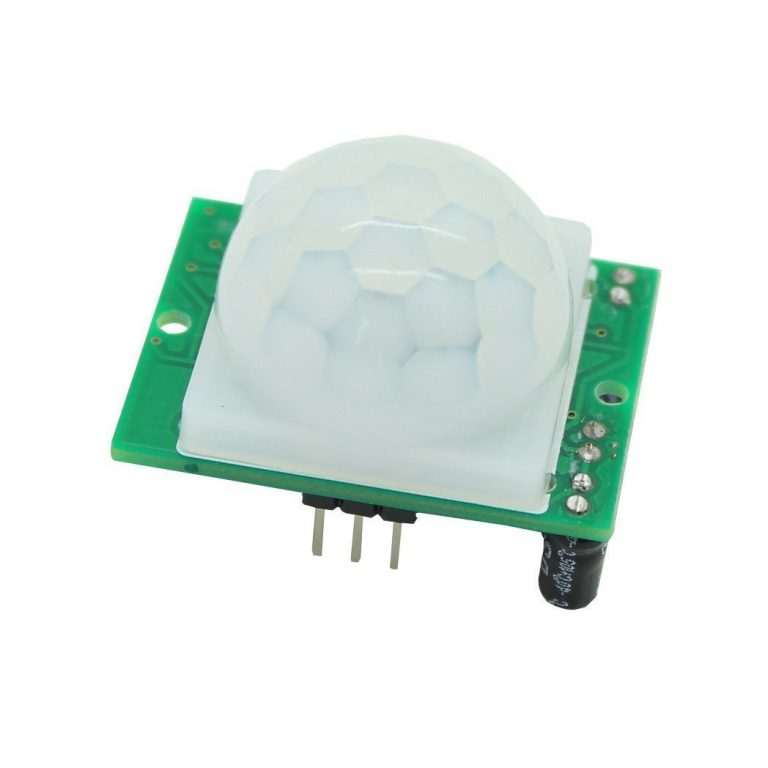
\includegraphics[width=50]{pictures/Bewegungssensor.jpg}
\caption{Bewegungssensor}
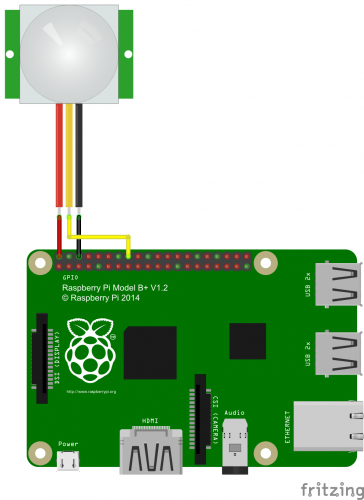
\includegraphics[width=80]{pictures/Bewegungssensor_Plan.png}
\caption{Schaltplan}

\subsection{Motion Control}
Um mehrere Ansichts Fenster auf dem SmartMirror zu besitzen und ziwschen denen auch navigieren zu können, wäre ein Motion-Control erforderlich. Dieser ermöglicht mit Gestiken, wie mit der Hand zur Seite wischen um die Seite zu wechseln, zu navigieren. Diese wären aber natürlich selber programmier- und konfigurierbar. 
Als Hardware für dieses Konzept wäre ein Entfernungsmessungssensor, wie der von Sharp der "Sharp Reflektierender Sensor- GP2Y0A21YK0F"*, ein Analog zu Digital Konverter, wie der von Microchip "8-Channel A/D Converter - MCP3008"*, und ein Breadboard erforderlich.
Der Entfernungsmessungssensor kann die Entfernung von Objekten, mithilfe von Infrarotstrahlen, die am Objekt reflektiert werden, ermitteln. Der Konverter wird benötigt, da der Raspberry Pi nur Digitale Ein- und Ausgänge besitzt und der Entfernungsmessungssensor Analogen Ausgänge besitzt. Das Breadboard wäre dafür da, um den Raspberry Pi und den Sensor über den Konverter zu verbinden.
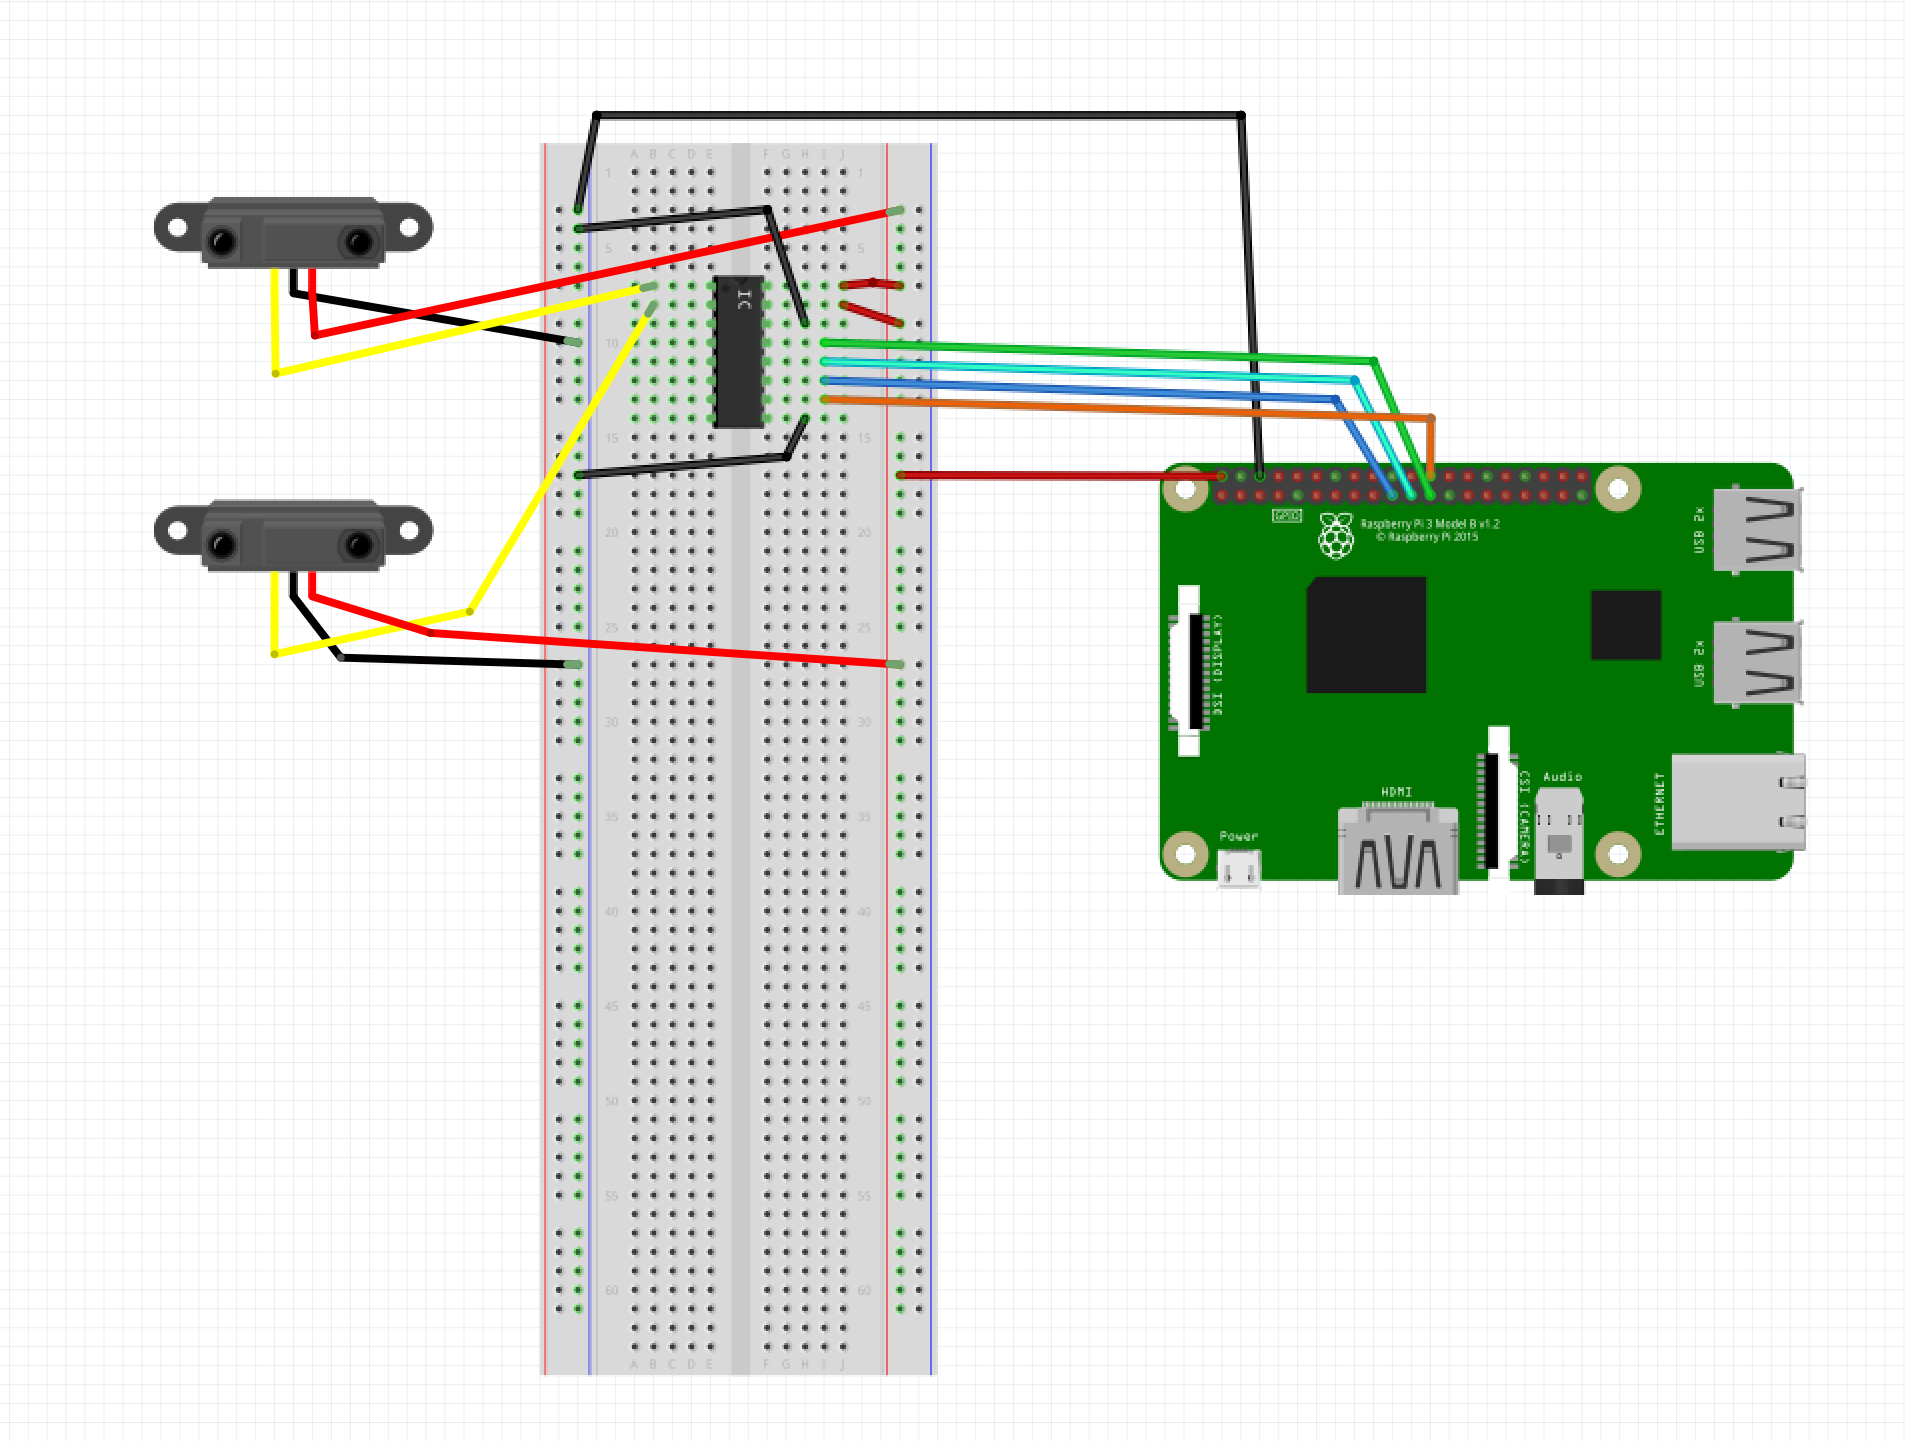
\includegraphics[]{pictures/Motion-Control_Plan.PNG}